\section{Study 2: frontier agents under the same judge}
\label{sec:agents}

\paragraph{Harness.} An agent receives the target only through tools and edits a model step by step. After every change, the harness assembles the CadQuery program, executes and checks it as in \cref{sec:protocol}, and reports build status, validity and executed IoU; the delivered answer is the best executed valid program, or, if no check of a valid program finished within the episode, the current program unverified (it is still re-judged offline like every other delivery). The \textbf{code} toolset is \texttt{describe\_target} (size, volume, flat-face directions and offsets), \texttt{section} (exact cross-sections of target and model), \texttt{evaluate}, \texttt{add\_code}, \texttt{remove\_step}, \texttt{list\_steps} and \texttt{finish}: it gives target inspection and execution feedback, so it is not an unaided language-model baseline. The \textbf{CADFit} toolset adds the optimizer's stages: direction detection, sketch extraction on a plane with line/arc fitting, extrusion and revolve fitting, section extrusion, and candidate management. Each episode has 40 tool calls and 30 minutes.

\paragraph{Models and runs.} Claude Opus~5.5 (\texttt{claude-opus-5-5}) and Sonnet~5.5 (\texttt{claude-sonnet-5-5}) run through the Anthropic Messages API with adaptive thinking at effort high, at most 32k output tokens per turn, the full conversation history, and no server-side fallback to another model. Each model runs three independent episodes per part and toolset on the 40 reserved parts; every delivered program is re-judged offline by the same replay and judge as the optimizer. These comparisons were specified after the optimizer study and are exploratory; intervals are nominal.

\begin{figure}[t]
\centering
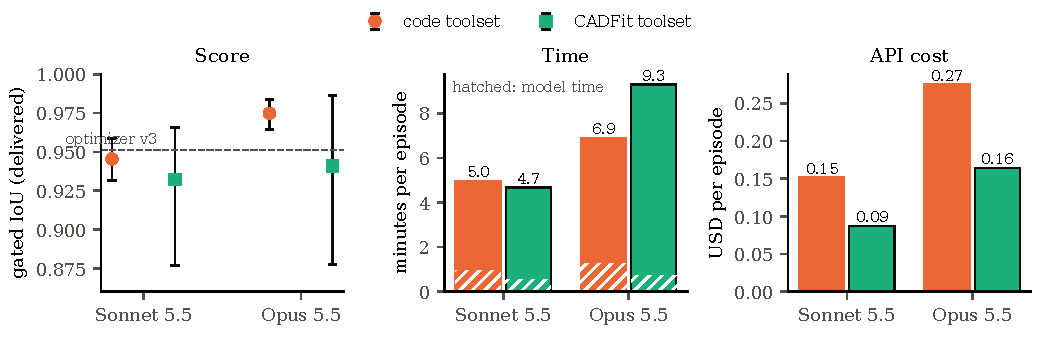
\includegraphics[width=\linewidth]{figures/closed.pdf}
\caption{Study 2, 40 reserved fresh2 parts, three episodes per part and condition. Left: gated IoU of the delivered program (mean over parts of the per-part mean; 95\% interval); dashed: the optimizer's v3 on the same parts. Middle: mean minutes per episode, hatched part waiting on the model. Right: mean API cost per episode. Runtime and cost are means without intervals.}
\label{fig:closed}
\end{figure}

\begin{table}[t]
\centering
\small
\caption{Study 2 against the optimizer on the same 40 parts (gated IoU, 95\% interval). Valid: delivered programs that build valid / episodes; no-output episodes ended at the deadline with nothing delivered. Differences are paired over parts (better/worse); exploratory.}
\label{tab:agents}
\setlength{\tabcolsep}{4pt}
\resizebox{\linewidth}{!}{%
\begin{tabular}{@{}lcccccc@{}}
\toprule
 & Gated IoU & 95\% interval & Valid & No output & Mean min & USD / episode \\
\midrule
Opus + code & \cOpusCode & \cOpusCodeCI & \cOpusCodeValid & \cOpusCodeNoOut & \cOpusCodeMin & \cOpusCodeCost \\
Opus + CADFit tools & \cOpusSkills & \cOpusSkillsCI & \cOpusSkillsValid & \cOpusSkillsNoOut & \cOpusSkillsMin & \cOpusSkillsCost \\
Sonnet + code & \cSonnetCode & \cSonnetCodeCI & \cSonnetCodeValid & \cSonnetCodeNoOut & \cSonnetCodeMin & \cSonnetCodeCost \\
Sonnet + CADFit tools & \cSonnetSkills & \cSonnetSkillsCI & \cSonnetSkillsValid & \cSonnetSkillsNoOut & \cSonnetSkillsMin & \cSonnetSkillsCost \\
\midrule
optimizer d0 / dx & \cPipeDZero{} / \cPipeDX & & & & & \\
optimizer v3 / + trim & \cPipeVThree{} / \cPipeTrim & \cPipeVThreeCI{} / \cPipeTrimCI & & & & \\
\midrule
Opus code $-$ v3 & \multicolumn{6}{l}{\cOpusCodeVsVThree{} \cOpusCodeVsVThreeCI, \cOpusCodeVsVThreeWL} \\
Opus code $-$ trim & \multicolumn{6}{l}{\cOpusCodeVsTrim{} \cOpusCodeVsTrimCI, \cOpusCodeVsTrimWL} \\
CADFit tools $-$ code & \multicolumn{6}{l}{Opus \cOpusSkillsVsCode{} \cOpusSkillsVsCodeCI; Sonnet \cSonnetSkillsVsCode{} \cSonnetSkillsVsCodeCI} \\
\bottomrule
\end{tabular}}
\end{table}

\paragraph{Results.} Opus with the code toolset scores \cOpusCode{} with \cOpusCodeValid{} valid deliveries (\cref{fig:closed}, \cref{tab:agents}). On the same parts the optimizer's v3 scores \cPipeVThree; the paired difference \cOpusCodeVsVThree{} \cOpusCodeVsVThreeCI{} excludes zero, while the difference from the optimizer with trim, \cOpusCodeVsTrim{} \cOpusCodeVsTrimCI, does not, so superiority over the full optimizer package is not established. Opus exceeds Sonnet with the code toolset by \cOpusVsSonnetCode{} \cOpusVsSonnetCodeCI, better on \cOpusVsSonnetCodeWL{} parts.

\paragraph{The optimizer's stages as tools.} With the CADFit toolset, the mean differences from code are \cOpusSkillsVsCode{} \cOpusSkillsVsCodeCI{} for Opus and \cSonnetSkillsVsCode{} \cSonnetSkillsVsCodeCI{} for Sonnet. All \cDeliveredValid{} programs the agents delivered are valid; the CADFit arms also contain \cOpusSkillsNoOut{} (Opus) and \cSonnetSkillsNoOut{} (Sonnet) episodes that reached the deadline with nothing delivered, on three parts, and these score zero. Offline validity is not the same as in-episode verification: \cValidUnverified{} valid deliveries had not completed an executed check within their episode.

\paragraph{Where the time goes.} Tool execution, not the model, dominates episodes: \texttt{add\_code}, whose cost is the executed check after every change, takes \cAddCodeShareLo--\cAddCodeShareHi\% of tool time in the code arms, and single calls of the CADFit stages reached \cMaxCall\,s. Mean minutes per episode are \cOpusCodeMin{} (Opus, code) to \cOpusSkillsMin{} (Opus, CADFit tools); the optimizer's v3 takes \hMinFortyVThree{} minutes per part on these parts, on different hardware and without API cost.
